\documentclass[12pt,a4paper]{article}
\usepackage[UTF8]{ctex}
\usepackage[backend=bibtex]{biblatex}
\usepackage{amsmath,amsthm,amssymb,graphicx,multirow,float,caption}
\usepackage{geometry}
\geometry{left=2.54cm, right=2.54cm, top=3.18cm, bottom=3.18cm}
\usepackage{enumitem}
\usepackage{subcaption,booktabs,diagbox}
\setenumerate[1]{itemsep=0pt,partopsep=0pt,parsep=\parskip,topsep=5pt}
\setitemize[1]{itemsep=0pt,partopsep=0pt,parsep=\parskip,topsep=5pt}
\setdescription{itemsep=0pt,partopsep=0pt,parsep=\parskip,topsep=5pt}
\usepackage{adjustbox}
\usepackage[graphicx]{realboxes}
\usepackage{rotating}

\usepackage{titlesec}

\newcommand{\be}[1]{
    \begin{equation}
        #1
    \end{equation}
}

\newcommand{\bfig}[3]{
    \begin{figure}[H]
        \centering
        \includegraphics[width=#1\textwidth]{#2}
        \caption{#3}
    \end{figure}
}

\titleformat{\section}%设置section的样式
{\raggedright\large\bfseries}%右对齐,4号字,加粗
{\thesection .\quad}%标号后面有个点
{0pt}%sep label和title之间的水平距离
{}%标题前没有内容

\title{\vspace{-4cm}\Large 液晶物性}  %文章标题
\author{\kaishu 学号:202111030007 \hspace{2cm} 姓名:郑晓旸}   %作者的名称
\date{}

\begin{document}
\maketitle

\begin{abstract}
    实验中完成了对液晶盒的光学测量和电光效应的测量. 光学部分, 测量得到液晶盒对偏振面的旋光角度$\beta=101.5°$, 双折射附加相位差$\delta \approx 2\pi$. 电光效应测量方面, 实验研究了常黑模式下, 电光响应曲线随频率的变化, 并在f=0.745Hz情况下测量了
曲线的关键参数. 实验研究了液晶驱动电压的开关频率, 驱动频率和驱动电压对光强曲线的影响, 在合适的条件下测量了电光响应时间. 实验在连续变化驱动电压时观察到了液晶的衍射现象, 并测量了能够稳定产生衍射现象的电压范围. 最后根据衍射图样计算了液晶光栅的光栅常数. 

\textbf{关键词: 液晶\quad 双折射\quad 电光响应}
\end{abstract}

\section{引言}
许多有机物都存在一种中介相, 加热到熔点时, 会熔融为浑浊的液体, 继续加热到清亮点会突然变成各向同性的清亮液体. 
在温度介于熔点和清亮点之间, 有机物具有强烈的各向异性的同时又具有流动性的相, 称之为液晶相. 液晶具有的各向异性性质, 尤其是电学, 光学, 磁学上的各向异性十分有趣, 因而受到细致深入的研究, 并逐渐走出实验室, 制成了现在生活中常见的液晶显示屏. 

本实验将对液晶盒进行研究. 液晶本身是各向异性物质, 可以研究其双折射特性; 液晶盒是对液晶分子进行均匀扭曲的产物, 具有旋光效应. 这两个效应都引起光线偏振态的改变. 
对液晶盒施加一定的电压, 可以研究液晶的电光响应性质, 包括响应曲线, 响应时间, 以及电压下的衍射曲线.
\section{原理}
\subsection{液晶的双折射}
光照射到各向异性晶体时, 会发生两个方向的折射: 当光的偏振方向垂直于光轴时, 折射率为o光折射率$n_{o}$, 且光线遵循折射定律; 光的偏振方向平行于光轴时, 折射率为e光折射率$n_{e}$, 光线不遵守折射定律. 当线偏振光的偏振方向与光轴成$\theta$角入射时, 两个偏振分量将经历不同的光程, 从而产生相位差: 
\be{\delta=\frac{2\pi}{\lambda}(n_{o}-n_{e})d}
其中$\lambda$是入射光的波长, d是光在晶体中行进的长度. 

通过控制d, 可以使晶体对特定波长的光线产生固定的光程差$\delta$. 视$\theta$的大小, $\delta$对光线的偏振结构的改变有不同的效果. 

$\delta=\pi/2$时, 若$\theta=\frac{\pi}{2}n$, 其中n为整数, 则出射仍然为线偏振光; 若$\theta=\pi/4$, 则出射为圆偏振光; 其余为椭圆偏振光. 

$\delta=\pi$时, 入射的线偏振光出射仍然为线偏振光, 只是偏振方向将与入射光关于光轴对称. 

\subsection{液晶盒的旋光效应}
实验用的液晶是向列相液晶, 液晶分子保持平行排列状态, 分子重心混乱无序, 一般只有双折射的性质. 通过均匀扭曲两个基片之间的液晶层, 制成的液晶盒, 将具有旋光性质. 
旋光性质来源于介质对左旋光和右旋光的折射率不同, 表现为入射的线偏振光偏振面的旋转. 旋转角度一般与旋光物质的厚度d成正比
\be{\theta=\alpha(\lambda)d}
就液晶盒而言, 它同时具有旋光和双折射的性质. 因为液晶分子方向的扭转, 入射面和出射面的光轴方向并不一致. 偏振方向平行或垂直于入射面光轴方向的入射光, 将经历旋光效应; 以其他线偏振光入射时, 会获得双折射效应
带来的附加相位差, 以椭圆偏振光, 圆偏振光或线偏振光等形式出射. 
\subsection{液晶的电光效应}
\subsubsection{电光响应曲线}
液晶在外电场的作用下, 分子取向将发生改变. 作用在液晶盒上, 则表现为随着施加在盒上的电压增大, 液晶分子的扭曲结构就会被破坏. 为便于观察, 需要固定入射光的偏振状态和出射光的检偏位置, 而将液晶盒的电压驱动作为变量. 实验中使用"常黑模式"进行研究, 即在无电压驱动时, 入射液晶盒的偏振光出射也是偏振光的同时, 
检偏器处于消光状态. 那么, 液晶盒的光学性质上的改变, 将表现为检偏器后出射光对消光状态的偏离. 

实验中涉及的物理量有两个, 一个自然是驱动电压$V(t)$, 由函数发生器产生, 一个是检偏器后的出射光的光强I(t), 用响应更为灵敏的光电二极管采集. 两个信号分别用示波器的CH1, CH2记录, 在此基础上能够得到I随V变化的曲线, 也就是待测的电光响应曲线. 
电光响应曲线的可预计特征是, 电压达到一定阈值以后, 会明显破坏液晶盒的旋光性, 出射光强显著偏离消光状态. 为此, 可以定义电光响应曲线的三个基本的物理量: 阈值电压(出射光强达到最大值的0.1), 饱和电压(出射光强达到最大值的0.9), 阈值锐度(饱和电压与阈值电压的比). 
\subsubsection{电光响应时间}
施加在液晶上的电压改变时, 液晶的状态弛豫到平衡态需要一定的时间, 这就是我们要测量的响应时间. 为测量响应时间, 
需要给液晶盒设置高低电平交替的周期电压; 高电平状态时, 为防止使用直流电损耗液晶盒的寿命, 实际上施加的是频率更高的高电平方波脉冲. 因此涉及到的物理量有三个, 驱动电压(高电平的电压), 驱动频率(高电平时脉冲的频率), 开关频率(高低电平交替的频率). 

由于电压上升和下降时电光响应曲线不同, 电光响应时间也不同, 分别对上升和下降的情况测量上升沿时间(光强由最小值上升到最大值的0.9所需时间), 下降沿时间(光强由最大值降到最大值的0.1所需时间).

\subsection{液晶的衍射}
施加在液晶盒上的低频电压达到一定大小后, 带电杂质的运动引起液晶分子的环流, 这些环流导致了液晶盒中液晶取向的周期变化, 引起折射率的周期变化, 从而能够形成光栅结构(威廉姆斯畴). 当电压进一步增大时, 可能会破坏已有的畴的结构. 因此, 只有在一定的电压范围内, 
才能观察到液晶的衍射现象. 可以通过光栅方程反推畴的光栅常数: 
\be{a\sin{\theta}=k\lambda}
其中a为光栅常数, $\theta$为衍射角, 整数k为衍射级次, $\lambda$为波长. 
\section{实验与结果分析}
\subsection{液晶的旋光与双折射现象}
由激光器出射的光是有着较高偏振度的光源, 调整起偏器至合适位置, 使得起偏器后是光强合适的线偏振光. 
在起偏器后使光线通过检偏器, 最后通过光电池检测光强, 结果如下表: 
\begin{table}[H]
    \centering
    \begin{tabular}{|cc|cc|}
    \hline
    \multicolumn{2}{|c|}{Imax}          & \multicolumn{2}{c|}{Imin}         \\ \hline
    \multicolumn{1}{|c|}{$\theta$} & I/mW   & \multicolumn{1}{c|}{$\theta$}  & I/uW \\ \hline
    \multicolumn{1}{|c|}{192°}  & 1.756 & \multicolumn{1}{c|}{282°}   & 2.8 \\ \hline
    \multicolumn{1}{|c|}{12.5°} & 1.757 & \multicolumn{1}{c|}{102.5°} & 2.9 \\ \hline
    \end{tabular}
    \caption{无液晶盒偏振情况测量}
    \end{table}
上表中记录了对起偏得到的线偏振光的偏振情况测量, 包括两次光强极大值时和两次消光时检偏器的角度$\theta$和光电池测得的光强I. 
两个光强最小值对应的检偏器角度相差180°, 光强最大值和最小值对应的角度相差90°, 符合预期. 偏振度计算为
\be{P=\frac{I_{max}}{I_{min}}=\frac{1.757}{2.8\times 10^{-3}}=627.5}

之后, 在起偏器和检偏器之间放入液晶盒. 在起偏器方向不变的情况下, 移动液晶盒直到出射光再次为线偏振光(称为二次消光). 由前面的原理分析知, 此时入射液晶盒的偏振光偏振方向与光轴垂直或平行. 
用检偏器记录此时的最大最小光强对应的角度如下表: 
\begin{table}[H]
    \centering
    \begin{tabular}{|cc|cc|}
    \hline
    \multicolumn{2}{|c|}{Imax}          & \multicolumn{2}{c|}{Imin}         \\ \hline
    \multicolumn{1}{|c|}{$\theta$} & I/mW   & \multicolumn{1}{c|}{$\theta$}  & I/uW \\ \hline
    \multicolumn{1}{|c|}{291.5°}  & 1.445 & \multicolumn{1}{c|}{23.5°}   & 3.1 \\ \hline
    \multicolumn{1}{|c|}{116°} & 1.475 & \multicolumn{1}{c|}{204°} & 3.5 \\ \hline
    \end{tabular}
    \caption{加入液晶盒偏振情况测量}
    \end{table}

两次出射时都是线偏振光, 在入射光偏振方向不变的情况下, 引起变化的是液晶盒的旋光性. 偏振面旋转了多少可以从消光处的角度计算得出(消光的判断比光强极值的判断更为准确): 
\be{\beta=\frac{1}{2}(204°-102.5°+360°-282°+23.5°)=101.5°}
这就是实验中使用的液晶盒引起的偏振面旋转的总量. 

为了进一步研究液晶盒的双折射性质, 在二次消光的基础上, 旋转液晶盒, 记录出射光极大值和极小值对应的角度. 
实验中发现, 尽管旋转了液晶盒以后, 出射光不再是线偏振光(通常是椭圆偏振光), 但极大值和极小值的角位置基本没变, 与表2中一致. 下面记录了
液晶盒的角度与最大光强和最小光强的关系: 
\begin{table}[H]
    \centering
    \begin{tabular}{|c|c|c|}
    \hline
    $\alpha$/° & Imax/mW & Imin/uW \\ \hline
    294     & 1.474   & 4.6     \\ \hline
    310     & 1.481   & 11.9    \\ \hline
    325     & 1.480   & 28.0    \\ \hline
    340     & 1.473   & 36.3    \\ \hline
    355     & 1.457   & 26.4    \\ \hline
    10      & 1.381   & 12.0    \\ \hline
    25      & 1.445   & 5.5     \\ \hline
    40      & 1.493   & 10.6    \\ \hline
    55      & 1.376   & 21.5    \\ \hline
    70      & 1.406   & 31.5    \\ \hline
    85      & 1.479   & 24.5    \\ \hline
    100     & 1.458   & 10.9    \\ \hline
    115     & 1.422   & 5.2     \\ \hline
    160     & 1.376   & 28.1    \\ \hline
    205     & 1.451   & 4.8     \\ \hline
    250     & 1.435   & 27.4    \\ \hline
    295     & 1.486   & 4.6     \\ \hline
    \end{tabular}
    \caption{旋转液晶盒后的偏振态测量}
    \end{table}
表中的$\alpha$是液晶盒的角度. $\alpha$变化的前180°每15°测量一次, 后180°每45°测量一次. 从最右侧消光列的数据可以明显看出, 最小光强以90°为变化周期, 每45°进行一次最大值和最小值的交替. 同时, 
最小光强相比于最大光强来说相当小, 几乎可以认为偏振状态经过双折射改变不大. 

为了解释这种变化情况和前面所述的光强极值的检偏器角度不变的情况, 需要考虑双折射效应. 不妨设入射的线偏振光的振幅为A, 从二次消光位置起液晶盒旋转角度$\alpha$后, 
偏振光正交分解为两个分量$A\sin{\alpha}$和$A\cos{\alpha}$两个分量, 经过双折射后在检偏方向投影, 得到
\be{I_{min}=A^2\sin{\alpha}^2\cos{\alpha}^2\left \langle (\cos{(\omega t) }-\cos{(\omega t -\delta)})^2 \right \rangle  =A^2\sin{\alpha}^2\cos{\alpha}^2(1-\cos{\delta})}

对于任意的$\delta$, 检偏方向不一定是最小值, 除非$\cos{\delta}=1$. 但又不是准确的相等, 这使得我们在实验中能观察到90°一次的周期变化, 而这恰好由前面$\sin{\alpha}^2\cos{\alpha}^2$决定. 因此, 我们得到结论, 实验中使用的液晶盒附加的相位差大致是$2\pi$, 或者换句话说, 双折射的影响很弱. 
\subsection{液晶的电光效应}
\subsubsection{液晶的电光响应曲线}
为了观察到电压的线性上升和线性下降时液晶盒的电光响应, 使用函数发生器驱动大致12V的三角波. 此时频率也成为了响应曲线的变量之一. 大致上, 电光响应曲线随频率的变化有三个阶段, 如下图所示: 
\bfig{0.8}{响应曲线.jpg}{常黑模式下响应曲线随频率的变化}
先定义物理量对比度为透过率的最大值与最小值的比, 即
\be{C=\frac{I_{max}}{I_{min}}}
于是可以发现, 在10Hz以下, 液晶的对比度比较大. 100Hz往上, 液晶的对比度极大地减小. 另一个特征是, 电压上升阶段和下降阶段的响应曲线并不重合. 频率较低时(<0.1Hz), 两个阶段的曲线几乎重合, 随着频率的逐渐增大, 两个曲线由中部向两边分开, 形成类似磁滞回线的结构. 
频率进一步增大, 液晶的对比度下降, 透过率的最小值上升, 电光响应曲线类似于一个"$\infty$"字, 并随着频率的增大扁平化. 当频率达到1000Hz的量级以后, 只有一条平线了, 即液晶盒的透过率对电压值不敏感, 可以理解为液晶盒响应跟不上电压的变化, 但螺旋结构依旧被破坏了. 在这个阶段, 随着频率的增大, 透过率的这条水平线也在逐渐下降, 趋于暗态, 即液晶分子保持未施加电压的状态, 螺旋结构来不及被破坏. 

为了得到准确的响应曲线的阈值电压, 饱和电压和阈值锐度, 需要选择频率较低的响应曲线进行测量. 
选取f=0.745Hz, 测得光强的饱和值(最大值)为33.8个单位, 对应的0.9和0.1为30.42和3.38个单位. 实际示波器的有效数字没有那么多, 选取最接近这两个值的光强值进行电压的测量. 由于阈值电压以后, 曲线的变化斜率很大, 这样测量的影响很小. 
测得上升阶段和下降阶段曲线的三个参数如下:
\begin{table}[H]
    \centering
    \begin{tabular}{|c|c|c|c|}
    \hline
       & $V_s$   & $V_{th}$  & $\beta$ \\ \hline
    上升 & 8.60 & 7.40 & 1.16 \\ \hline
    下降 & 8.60 & 5.60 & 1.54 \\ \hline
    \end{tabular}
    \caption{f=0.745Hz响应曲线参数}
    \end{table}
0.745Hz是实验中为了测量效率选取的频率. 在此基础上考虑低频极限的参数, 应有$V_s=8.6V, V_{th}\approx 6V, \beta\approx 1.43$. 

\subsection{液晶的电光响应时间}
实验中先定性研究了施加电压的开关频率, 驱动频率与驱动电压对光强曲线I(t)的影响. 概括一下, 这些参数影响图形的这些参数: 
\bfig{0.7}{响应时间.jpg}{光强变化曲线示意图}
示意图中下方是施加的方波. 图中标记的几个图形特征: 1为饱和电压的陡峭情况, 2为饱和电压维持时间, 3为光强的最小值, 4为不同光强相邻峰的最小距离. 
一般来说, 高电平处的驱动频率越大, 1处的陡峭程度就越小, 反之陡峭程度就越大. 开关频率越大, 3处光强就来不及弛豫到最小值(暗态), 最小值就会越大, 反之则会越小. 驱动电压越大, 2处维持饱和光强的阶段就越长, 反之可能电压尚未达到饱和阶段即下降. 

之后, 选取合适的开关频率, 驱动频率和驱动电压, 使得曲线的2处足够长, 1处陡峭足够小, 2处光强比较小的情况, 进行相应时间的测量. 从-5.6ms到63.6ms的完整周期内, 几个关键时间点如下: 
\begin{table}[H]
    \centering
    \begin{tabular}{|c|c|c|c|c|c|}
    \hline
    t&-5.6 & 1.2 & 28.0 & 38.8 & 63.6 \\ \hline
    事件&a    & b   & c  & d    & e    \\ \hline
    \end{tabular}
    \caption{一次光强变化曲线中的关键节点. 时间单位: ms. }
    \end{table}
其中a为起始点, 此时刚好进入高电平状态, b为第一次达到0.9倍光强最大值的时刻, c为电压开始下降的时刻(进入低电平的时刻), d为电压下降到0.1倍最大值的时刻, e为下一次进入高电平的时刻. 
则
\begin{align}
&T_{on}=t_{b}-t_{a}=6.8ms\\
&T_{off}=t_{d}-t_{c}=10.8ms\\
&T=T_{on}+T_{off}=17.6ms
\end{align}
上升沿时间为6.8ms, 下降沿时间为10.8ms, 全过程响应时间为17.6ms. 
\bfig{0.5}{响应时间示意.jpg}{实验时测量图}
\subsection{液晶的衍射}
置液晶驱动电源为连续状态, 此时输出的直流电, 电压值可以通过旋钮调整. 实验中使用的仪器无法在停止旋转旋钮后, 电压值立刻稳定下来, 中间的这段时间对液晶分子的环流状态可能造成破坏. 事实上, 当带电杂质在电场驱动下的运动达到平衡以后, 液晶分子的环流将会消失, 将观察不到衍射现象. 
而实验中的确观察到了停止旋钮后, 电压还未稳定下来, 衍射现象逐渐消失的情况. 为了确定某个电压值, 还需要反复调整. 然而由前面的"磁滞回线"图, 调整历史会对液晶的状态造成影响. 因此, 实验数据中只能得到衍射现象比较稳定的电压范围: 4.02V-6.14V. 

该电压值比较偏离前面测出的阈值电压和饱和电压. 如果液晶驱动电源旋钮和电压的响应更好的话, 可以比较缓慢但连续地调整驱动电压, 以观察衍射现象的出现和消失, 将观察到电压上升阶段和下降阶段临界电压的不同. 若在显微镜下进行观察, 测量也会更加准确. 

在能够稳定观察到衍射的情况下, 调整白屏至合适位置, 对衍射斑进行测量. 实验中能观察到中心对称的五个光斑. 光屏置于在液晶盒后l=10.4cm处, 光斑位置的示意图如下: 
\bfig{0.5}{液晶衍射示意图.jpg}{液晶衍射测量示意图}
光斑的尺度大约在0.5cm, 0级和1级光斑间距为$d=1.25cm$, 并取激光的波长$\lambda=650nm$, 于是代入公式(3), 有
\be{a=\frac{\lambda \sqrt{d^2+l^2}}{d}=5.4(1)\mu m}
这里的不确定度是用$u(d)=0.2cm$计算的, 这相应于识别光斑位置的不确定度. 
\section{总结}
实验中完成了对液晶盒的光学测量和电光效应的测量. 光学部分, 测量得到液晶盒对偏振面的旋光角度$\beta=101.5°$, 双折射附加相位差$\delta \approx 2\pi$. 电光效应测量方面, 实验研究了常黑模式下, 电光响应曲线随频率的变化, 并在f=0.745Hz情况下测量了
曲线的关键参数. 实验研究了液晶驱动电压的开关频率, 驱动频率和驱动电压对光强曲线的影响, 在合适的条件下测量了电光响应时间. 实验在连续变化驱动电压时观察到了液晶的衍射现象, 并测量了能够稳定产生衍射现象的电压范围. 最后根据衍射图样计算了液晶光栅的光栅常数$a=5.4\mu m$. 

\section{附录: 原始数据}
\begin{figure}[H]
    \centering
    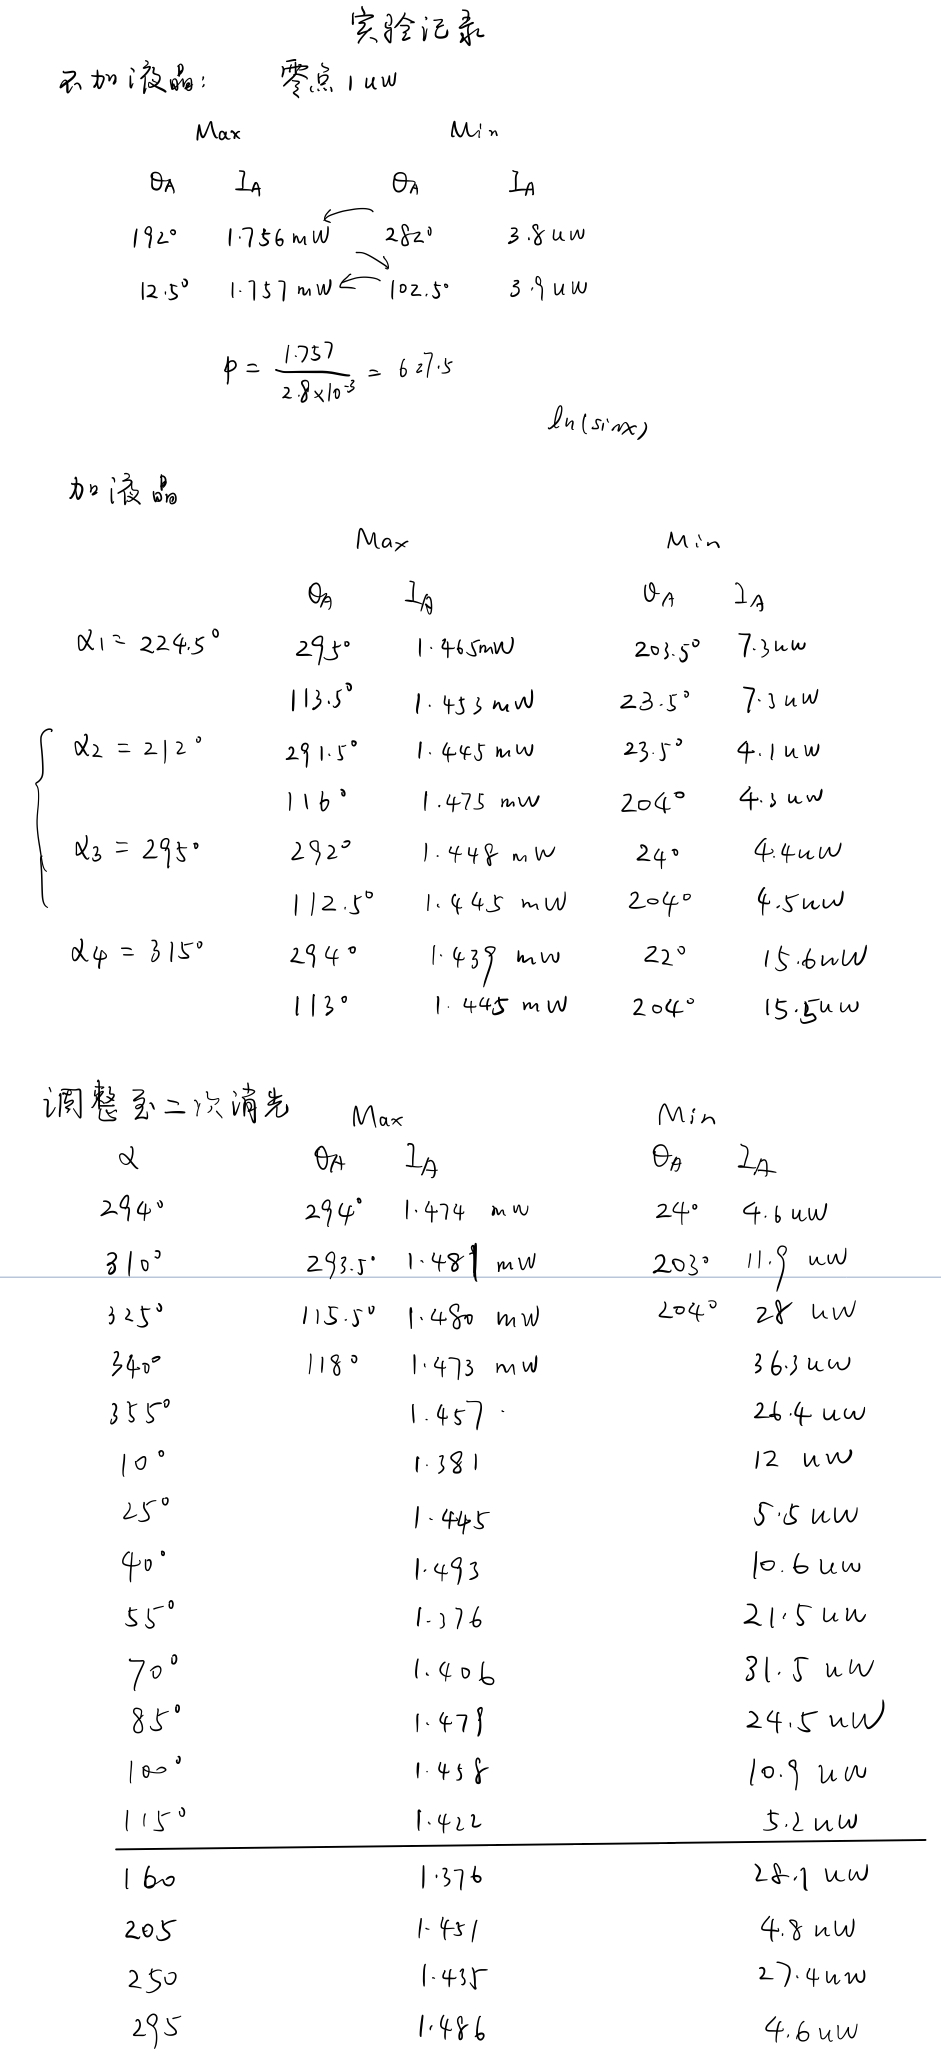
\includegraphics[width=0.5\textwidth]{数据1.jpg}
\end{figure}
\begin{figure}[H]
    \centering
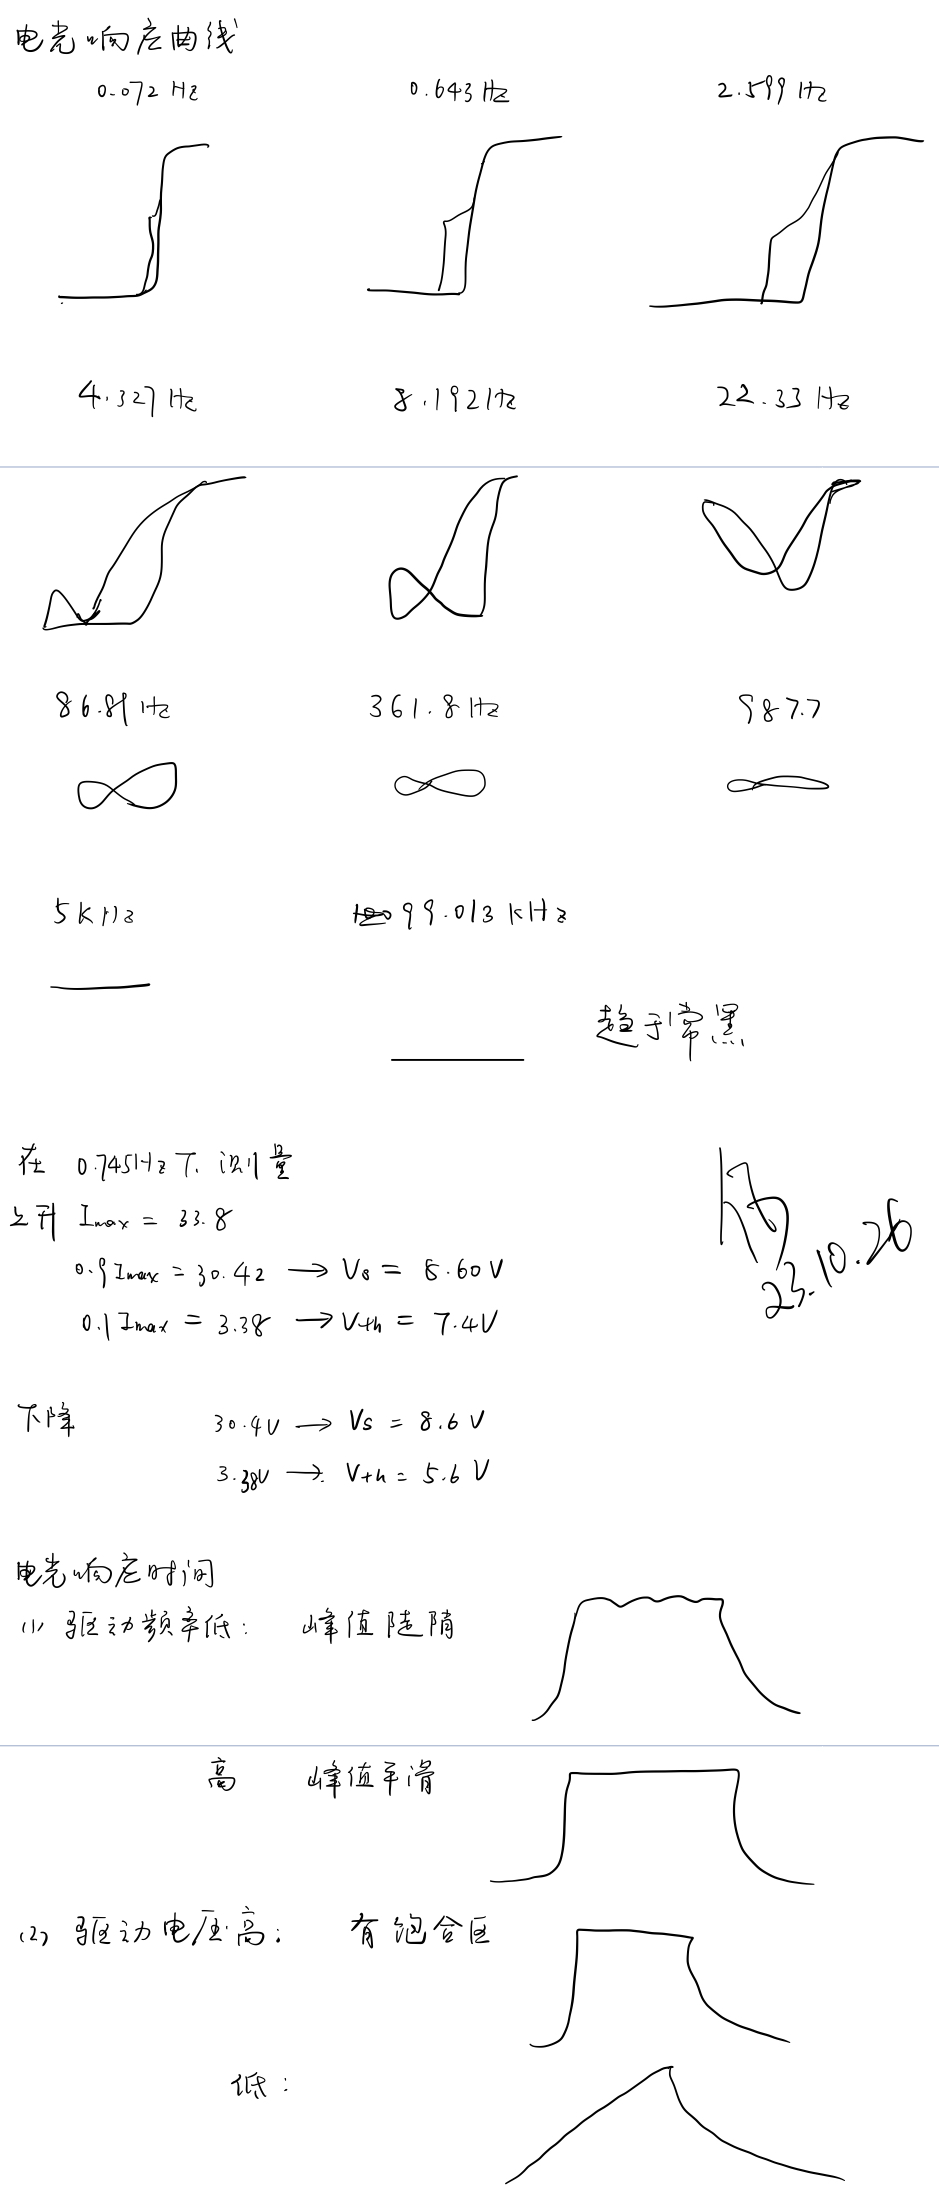
\includegraphics[width=0.5\textwidth]{数据2.jpg}
\end{figure}
\begin{figure}[H]
    \centering
    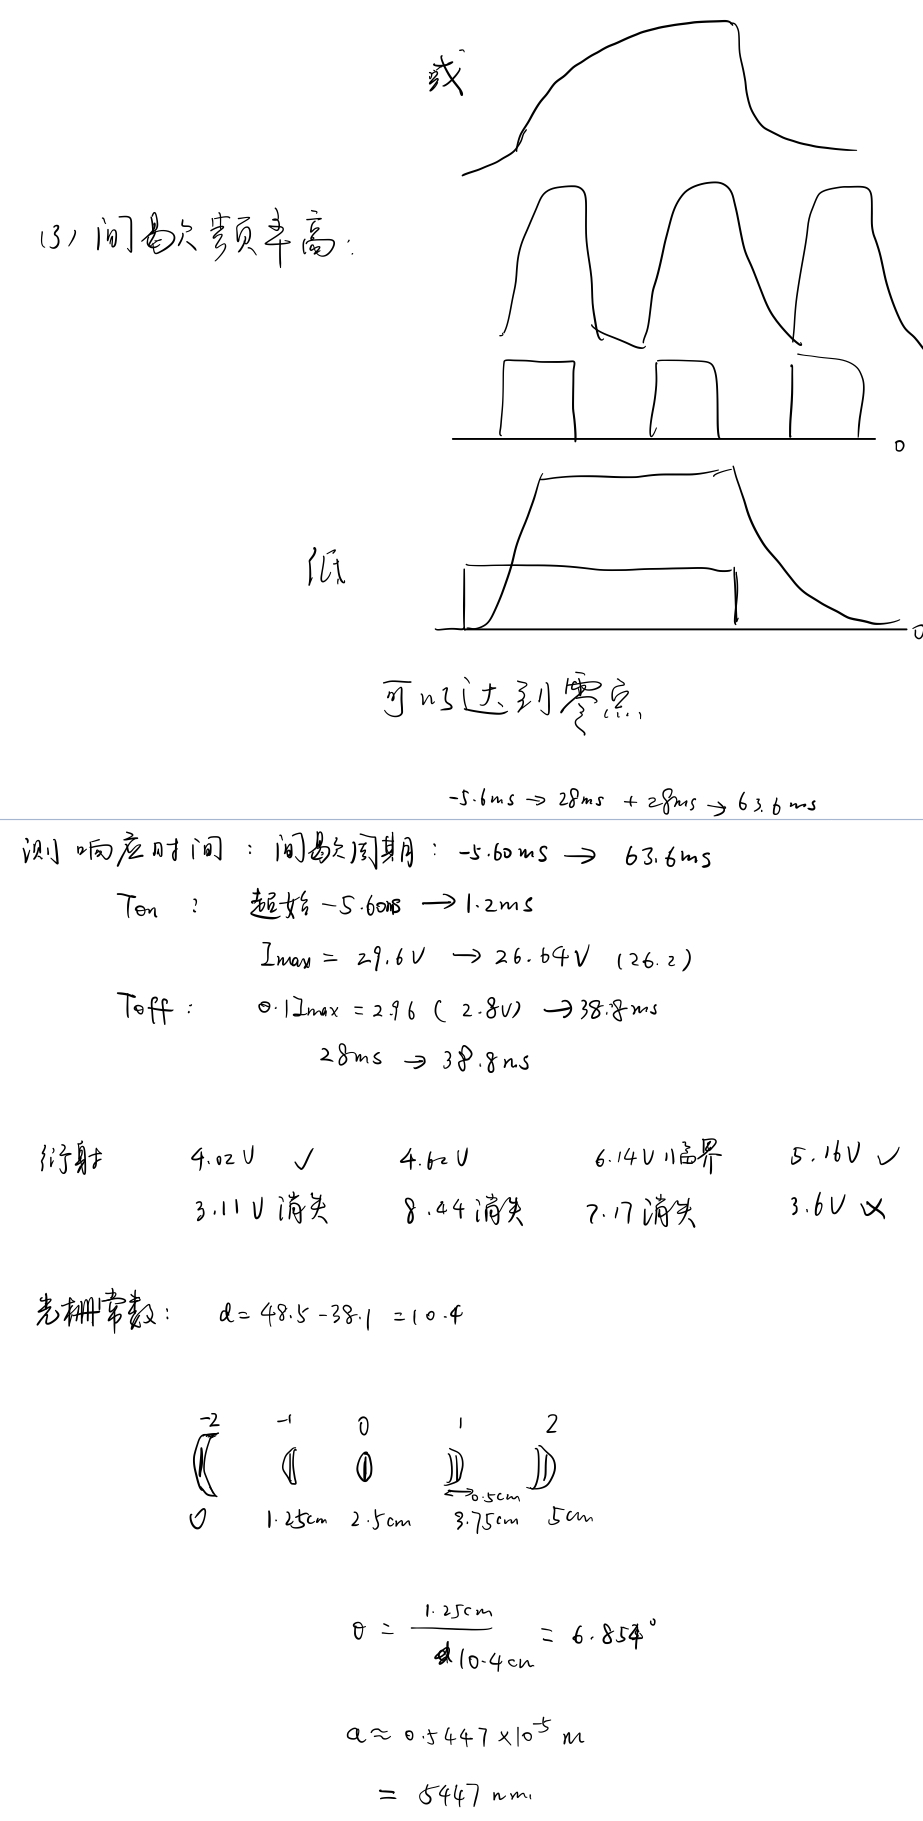
\includegraphics[width=0.5\textwidth]{数据3.jpg}
\end{figure}
\end{document}